%----------------------------------------------------------------------------------------
%	PACKAGES AND THEMES
%----------------------------------------------------------------------------------------
\pdfoutput=1
\documentclass[swedish, english]{beamer}



\usepackage[utf8]{inputenc}
%\usepackage[scaled]{helvet} %helvetica i sliden blir bra
\usepackage[T1]{fontenc}

\usepackage{graphicx} % Allows including images
\usepackage{booktabs} % Allows the use of \toprule, \midrule and \bottomrule in tables
%\usepackage{comment}
%\usepackage[swedish,english]{babel}
\usepackage{graphicx}
\usepackage{graphics}
%\usepackage{units}
\usepackage{epstopdf}
\usepackage{tikz}
\usepackage{eso-pic}
\usepackage{wallpaper} %For background pictures
\usepackage{multimedia}
\usepackage{media9}

\usepackage{physics}
\usepackage{cancel}
\usefonttheme[onlymath]{serif}

\graphicspath{ 
{figures/} %path to figures
}



\mode<presentation> {

% The Beamer class comes with a number of default slide themes
% which change the colors and layouts of slides. Below this is a list
% of all the themes, uncomment each in turn to see what they look like.

\usetheme{default}


% As well as themes, the Beamer class has a number of color themes
% for any slide theme. Uncomment each of these in turn to see how it
% changes the colors of your current slide theme.

\usecolortheme{beaver}

}



\newcommand{\swapcommands}[2]{ %This command swaps two commands.
  \let\temp#1
  \let#1#2
  \let#2\temp
}
\swapcommands{\phi}{\varphi}
\swapcommands{\epsilon}{\varepsilon}



\renewcommand{\thefootnote}{\fnsymbol{footnote}}
\newcommand{\ee}{\mathrm{e}}

%----------------------------------------------------------------------------------------
%	TITLE PAGE
%----------------------------------------------------------------------------------------



\title[Swings and Biorhythms]{Parametrically driven oscillators}
\subtitle{} % optional
\author{Leon Avery \and Andréas Sundström} % [short author (optional)]{many authors}
\institute[UW]{University of Waterloo}
\date{November 28, 2016}

%\date{\vspace{-0.25cm}\today}




\begin{document}

\begin{frame}[plain]
\linethickness{0.075mm}
  \titlepage
\end{frame}
% }




%%%%%%%%%%%%%%%%%%%%%%%%%%%%%%%%%%%%%%%%%%%%%%%%


% \begin{frame} %A frame with table of contents
% \frametitle{Contents}
% \tableofcontents
% \end{frame}



%\section{Overview}

\begin{frame}
\frametitle{Outline}

\begin{columns}[c]
\column{.5\textwidth} % Left column and width
\textbf{Swing}
\begin{itemize}
\item Governing equation
\item Physical explanation
\item Look at a solution
\item Comparison with numerical solution
\end{itemize}


\column{.5\textwidth} % Right column and width
\textbf{Circadian Rhythms}
\begin{itemize}
\item Explain the biology
\item Entrainment
\item Phase reduction technique
\item Phase response curve
\item Robustness
\end{itemize}

\end{columns}
\end{frame}



%\section{How to pump a swing}
%\subsection{The equation of motion}
\begin{frame}
\frametitle{Parametric forcing as a model for a child’s swing}

\begin{columns}[c]

\column{.4\textwidth} % Left column and width
\centerline{
\resizebox{.7\textwidth}{!}{
\input{figures/pendulum.pdf_t}}
}

\column{.7\textwidth} % Right column and width
\begin{itemize}
% \item Simple model:
% $l(t) = \bar{l}[1+\epsilon\cos(\omega t)]$.
\item Non-dimensionalized equation of motion:
$r\ddot\phi + 2\dot{r}\dot\phi + \eta^2\sin(\phi)=0$.\\
\vspace{5mm}

\item $r(t)=\frac{l(t)}{l_0}$
\item $\eta=\frac{\omega_0}{\omega}$ 
\begin{itemize}
\item Relates the forcing frequency to
the free-running frequency of the swing.
\end{itemize}
\end{itemize}

\end{columns}
\end{frame}


%\subsection{Energy of the swing}
% \begin{frame}
% \frametitle{The swing energy}
% The energy:
% \[
% E=\frac{1}{2}\qty[\dot{r}^2 + r^2\dot{\phi}^2]
% +\eta^2\qty[1-r\cos(\phi)].
% \] 

% More interesting is
% \[
% \dv{E}{t}
% =\dot{r}\ddot{r}+r\dot\phi\qty(r\ddot\phi + \dot{r}\dot\phi + \eta^2\sin\phi) 
% -\eta^2\dot{r}\cos\phi.
% \]

 
% \end{frame}


%\subsection{Physical interpretations}
\begin{frame}
\frametitle{Physical interpretation}
We have 
\[
\dv{E}{t}
=\dot{r}\ddot{r} - \dot{r}\qty(r\dot{\phi}^2 + \eta^2\cos\phi).
\]
%by using the EOM.
\vspace{11pt}

Study this over one cycle:
\begin{itemize}
\item The term $\dot{r}\ddot{r}$ disappears.
\item The two other terms corresponds to the \emph{centrifugal} and
\emph{gravitational} force.
\vspace{6pt}
\item By doing work against these forces, the child can pump energy
into the swing
\end{itemize}
\end{frame}

\begin{frame}
\frametitle{Physical interpretation}
\[
\dv{E}{t}
=\dot{r}\ddot{r} - \dot{r}\qty(r\dot{\phi}^2 + \eta^2\cos\phi).
\]

\vspace{11pt}
Optimal forcing:
\begin{itemize}
\item Abruptly stand up when $\phi=0$,
\item then abruptly sit down when $\phi$ is at its maximum.
\end{itemize}

This corresponds to having $\omega=2\omega_0$, i.e. $\eta=\frac{1}{2}$.

\end{frame}


\begin{frame}
\frametitle{Studying a solution, using energy}
The energy gained over one cycle:
\[
\Delta{E}=\int_0^{4\pi}\dv{E}{t}\dd{t}
= - \int_0^{4\pi}\dot{r}\qty(r\dot{\phi}^2 + \frac{1}{4}\cos\phi) \dd{t}.
\]
\vspace{6pt}

\begin{itemize}
\item Let the forcing function $r(t)=1+\epsilon\cos(t+t_0)$, \;\;$\epsilon\ll1$.
\item First order approximation: $\phi(t)=a_0\cos(t/2)$, is not
affected over the cycle.
%\item Both 
\end{itemize}
\end{frame}


\begin{frame}
\frametitle{Studying a solution, using energy}
The energy gained over one cycle becomes
\[
\Delta{E}=-3\pi\epsilon E_0\sin(t_0),
\]
where $E_0=a_0^2/8$.
\vspace{6pt}

\begin{itemize}
\item Choose $t_0=-\pi/2$.
\item Resulting in $r(t)=1+\epsilon\sin(t)$.
\end{itemize}

\begin{itemize}
\item Note: $E(t=4\pi)=(1+3\pi\epsilon)E(0)$ only depends on the
initial energy.
\end{itemize}
\end{frame}


\begin{frame}
\frametitle{Studying a solution, using energy}
Reasonable to assume exponential behavior
\[
E(t)=E_0\exp(\ln(1+3\pi\epsilon)\frac{t}{4\pi})
\approx E_0\ee^{\frac{3}{4}\epsilon t}.
\]

Or in terms of the angle
\[
\phi(t)\approx a_0\ee^{\frac{3}{8}\epsilon t}
\cos(t/2).
\]
\end{frame}

\begin{frame}
\frametitle{Studying a solution, using the method of multiple scales}
\[
\phi(t)\approx a_0\ee^{\frac{3}{8}\epsilon t}
\cos(t/2).
\]
\vspace{16pt}

We get exactly the same first order solution if we were to use the
\emph{Method of multiple scales}.


\end{frame}



% \begin{frame}
% \frametitle{Studying a solution, using the method of multiple scales}
% Introduce $\tau=\epsilon t$.
% New EOM:
% \[
% \begin{aligned}
% \phi_{tt}+2\epsilon\phi_{t\tau}+\epsilon^2\phi_{\tau\tau}+\eta^2\phi
% =&
% \epsilon\qty[-2\cos(t)(\phi_t+\epsilon\phi_\tau)+\eta^2\sin(t)\phi]
% \\&\hspace{-8pt}
% +\epsilon^2\qty[2\sin(t)\phi_t-2\eta^2\sin^2(t)\phi]
% +\order{\epsilon^3},
% \end{aligned}
% \]
% with initial conditions $\phi(0, 0)=a_0$ and $\phi_t(0,
% 0)+\epsilon\phi_\tau(0, 0)=0$.

% \vspace{11pt}
% \begin{itemize}
% \item Next step is to expand: 
% $\phi=\phi_0+\epsilon\phi_1+\epsilon^2\phi_2+\ldots$
% \item We will again use $\eta=1/2$.
% \end{itemize}


% \end{frame}


% \begin{frame}
% \frametitle{Studying a solution, using the method of multiple scales}
% The $\order{1}$ problem:
% \[\phi_{0, tt}+\frac{1}{4}\phi_0=0,\] 
% with $\phi_0(0,0)=a_0$ and $\phi_{0, t}(0,0)=0$.

% \vspace{11pt}
% The solution
% \[ \phi_0(t, \tau)=A_0(\tau)\cos(t/2)+B_0(\tau)\sin(t/2),\]
% where $A_0(0)=a_0$ and $B_0(0)=0$.
% \end{frame}


% \begin{frame}
% \frametitle{Studying a solution, using the method of multiple scales}
% \begin{itemize}
% \item The $\order{\epsilon}$ problem has secular terms.
% \item To eliminate these secular terms we get the two ODEs
% \[\begin{cases}
% A_{0,\,\tau}-\frac{3}{8}A_0=0\qcomma&A_0(0)=a_0,\\
% B_{0,\,\tau}+\frac{3}{8}B_0=0\qcomma&B_0(0)=0,
% \end{cases}\]

% \end{itemize}
% \vspace{11pt}
% The $\order{1}$ solution becomes
% \[ \phi_0(t, \tau)=a_0\ee^{\frac{3}{8}\tau}\cos(t/2),\]
% which is preciesly what we had before.
% \end{frame}


\begin{frame}
\frametitle{Numerical solutions}


\centerline{
\resizebox{1.1\textwidth}{!}{
% GNUPLOT: LaTeX picture with Postscript
\begingroup
  \makeatletter
  \providecommand\color[2][]{%
    \GenericError{(gnuplot) \space\space\space\@spaces}{%
      Package color not loaded in conjunction with
      terminal option `colourtext'%
    }{See the gnuplot documentation for explanation.%
    }{Either use 'blacktext' in gnuplot or load the package
      color.sty in LaTeX.}%
    \renewcommand\color[2][]{}%
  }%
  \providecommand\includegraphics[2][]{%
    \GenericError{(gnuplot) \space\space\space\@spaces}{%
      Package graphicx or graphics not loaded%
    }{See the gnuplot documentation for explanation.%
    }{The gnuplot epslatex terminal needs graphicx.sty or graphics.sty.}%
    \renewcommand\includegraphics[2][]{}%
  }%
  \providecommand\rotatebox[2]{#2}%
  \@ifundefined{ifGPcolor}{%
    \newif\ifGPcolor
    \GPcolortrue
  }{}%
  \@ifundefined{ifGPblacktext}{%
    \newif\ifGPblacktext
    \GPblacktexttrue
  }{}%
  % define a \g@addto@macro without @ in the name:
  \let\gplgaddtomacro\g@addto@macro
  % define empty templates for all commands taking text:
  \gdef\gplbacktext{}%
  \gdef\gplfronttext{}%
  \makeatother
  \ifGPblacktext
    % no textcolor at all
    \def\colorrgb#1{}%
    \def\colorgray#1{}%
  \else
    % gray or color?
    \ifGPcolor
      \def\colorrgb#1{\color[rgb]{#1}}%
      \def\colorgray#1{\color[gray]{#1}}%
      \expandafter\def\csname LTw\endcsname{\color{white}}%
      \expandafter\def\csname LTb\endcsname{\color{black}}%
      \expandafter\def\csname LTa\endcsname{\color{black}}%
      \expandafter\def\csname LT0\endcsname{\color[rgb]{1,0,0}}%
      \expandafter\def\csname LT1\endcsname{\color[rgb]{0,1,0}}%
      \expandafter\def\csname LT2\endcsname{\color[rgb]{0,0,1}}%
      \expandafter\def\csname LT3\endcsname{\color[rgb]{1,0,1}}%
      \expandafter\def\csname LT4\endcsname{\color[rgb]{0,1,1}}%
      \expandafter\def\csname LT5\endcsname{\color[rgb]{1,1,0}}%
      \expandafter\def\csname LT6\endcsname{\color[rgb]{0,0,0}}%
      \expandafter\def\csname LT7\endcsname{\color[rgb]{1,0.3,0}}%
      \expandafter\def\csname LT8\endcsname{\color[rgb]{0.5,0.5,0.5}}%
    \else
      % gray
      \def\colorrgb#1{\color{black}}%
      \def\colorgray#1{\color[gray]{#1}}%
      \expandafter\def\csname LTw\endcsname{\color{white}}%
      \expandafter\def\csname LTb\endcsname{\color{black}}%
      \expandafter\def\csname LTa\endcsname{\color{black}}%
      \expandafter\def\csname LT0\endcsname{\color{black}}%
      \expandafter\def\csname LT1\endcsname{\color{black}}%
      \expandafter\def\csname LT2\endcsname{\color{black}}%
      \expandafter\def\csname LT3\endcsname{\color{black}}%
      \expandafter\def\csname LT4\endcsname{\color{black}}%
      \expandafter\def\csname LT5\endcsname{\color{black}}%
      \expandafter\def\csname LT6\endcsname{\color{black}}%
      \expandafter\def\csname LT7\endcsname{\color{black}}%
      \expandafter\def\csname LT8\endcsname{\color{black}}%
    \fi
  \fi
  \setlength{\unitlength}{0.0500bp}%
  \begin{picture}(9636.00,4534.00)%
    \gplgaddtomacro\gplbacktext{%
      \csname LTb\endcsname%
      \put(744,768){\makebox(0,0)[r]{\strut{}$-1$}}%
      \put(744,2507){\makebox(0,0)[r]{\strut{}$0$}}%
      \put(744,4245){\makebox(0,0)[r]{\strut{}$1$}}%
      \put(888,528){\makebox(0,0){\strut{} 0}}%
      \put(1471,528){\makebox(0,0){\strut{} 100}}%
      \put(2054,528){\makebox(0,0){\strut{} 200}}%
      \put(2637,528){\makebox(0,0){\strut{} 300}}%
      \put(3219,528){\makebox(0,0){\strut{} 400}}%
      \put(3802,528){\makebox(0,0){\strut{} 500}}%
      \put(4385,528){\makebox(0,0){\strut{} 600}}%
      \put(192,2506){\rotatebox{-270}{\makebox(0,0){\strut{}Original EOM}}}%
      \put(2636,168){\makebox(0,0){\strut{}$t$}}%
    }%
    \gplgaddtomacro\gplfronttext{%
      \csname LTb\endcsname%
      \put(2530,3995){\makebox(0,0)[r]{\strut{}$\phi(t)$}}%
      \csname LTb\endcsname%
      \put(2530,3755){\makebox(0,0)[r]{\strut{}$\pm a_0\exp(3\epsilon{t}/8)$}}%
    }%
    \gplgaddtomacro\gplbacktext{%
      \csname LTb\endcsname%
      \put(5562,768){\makebox(0,0)[r]{\strut{}$-1$}}%
      \put(5562,2507){\makebox(0,0)[r]{\strut{}$0$}}%
      \put(5562,4245){\makebox(0,0)[r]{\strut{}$1$}}%
      \put(5706,528){\makebox(0,0){\strut{} 0}}%
      \put(6289,528){\makebox(0,0){\strut{} 100}}%
      \put(6872,528){\makebox(0,0){\strut{} 200}}%
      \put(7455,528){\makebox(0,0){\strut{} 300}}%
      \put(8037,528){\makebox(0,0){\strut{} 400}}%
      \put(8620,528){\makebox(0,0){\strut{} 500}}%
      \put(9203,528){\makebox(0,0){\strut{} 600}}%
      \put(5010,2506){\rotatebox{-270}{\makebox(0,0){\strut{}Linearized EOM}}}%
      \put(7454,168){\makebox(0,0){\strut{}$t$}}%
    }%
    \gplgaddtomacro\gplfronttext{%
      \csname LTb\endcsname%
      \put(7348,3995){\makebox(0,0)[r]{\strut{}$\phi_\text{lin}(t)$}}%
      \csname LTb\endcsname%
      \put(7348,3755){\makebox(0,0)[r]{\strut{}$\pm a_0\exp(3\epsilon{t}/8)$}}%
    }%
    \gplbacktext
    \put(0,0){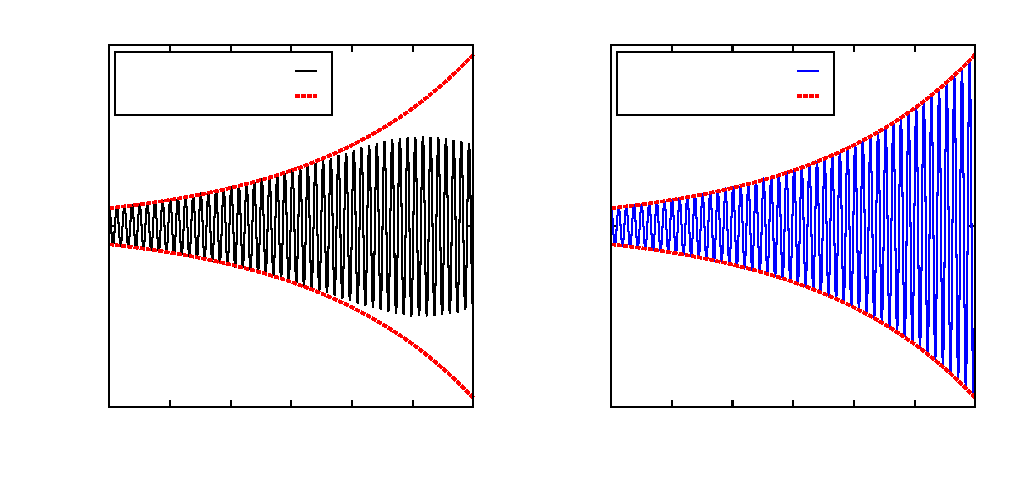
\includegraphics{swing_sim}}%
    \gplfronttext
  \end{picture}%
\endgroup
}
}


\begin{columns}
\column{.5\textwidth}
\hspace{25pt}
$\displaystyle
\ddot\phi + 2\frac{\dot{r}}{r}\dot\phi + \frac{\eta^2}{r}\sin(\phi)=0
$
\column{.5\textwidth}
\hspace{22pt}
$ \displaystyle
\ddot\phi + 2\frac{\dot{r}}{r}\dot\phi + \frac{\eta^2}{r}\phi=0 
$
\end{columns}
% \centerline{
% \resizebox{.7\textwidth}{!}{
% % GNUPLOT: LaTeX picture with Postscript
\begingroup
  \makeatletter
  \providecommand\color[2][]{%
    \GenericError{(gnuplot) \space\space\space\@spaces}{%
      Package color not loaded in conjunction with
      terminal option `colourtext'%
    }{See the gnuplot documentation for explanation.%
    }{Either use 'blacktext' in gnuplot or load the package
      color.sty in LaTeX.}%
    \renewcommand\color[2][]{}%
  }%
  \providecommand\includegraphics[2][]{%
    \GenericError{(gnuplot) \space\space\space\@spaces}{%
      Package graphicx or graphics not loaded%
    }{See the gnuplot documentation for explanation.%
    }{The gnuplot epslatex terminal needs graphicx.sty or graphics.sty.}%
    \renewcommand\includegraphics[2][]{}%
  }%
  \providecommand\rotatebox[2]{#2}%
  \@ifundefined{ifGPcolor}{%
    \newif\ifGPcolor
    \GPcolortrue
  }{}%
  \@ifundefined{ifGPblacktext}{%
    \newif\ifGPblacktext
    \GPblacktexttrue
  }{}%
  % define a \g@addto@macro without @ in the name:
  \let\gplgaddtomacro\g@addto@macro
  % define empty templates for all commands taking text:
  \gdef\gplbacktext{}%
  \gdef\gplfronttext{}%
  \makeatother
  \ifGPblacktext
    % no textcolor at all
    \def\colorrgb#1{}%
    \def\colorgray#1{}%
  \else
    % gray or color?
    \ifGPcolor
      \def\colorrgb#1{\color[rgb]{#1}}%
      \def\colorgray#1{\color[gray]{#1}}%
      \expandafter\def\csname LTw\endcsname{\color{white}}%
      \expandafter\def\csname LTb\endcsname{\color{black}}%
      \expandafter\def\csname LTa\endcsname{\color{black}}%
      \expandafter\def\csname LT0\endcsname{\color[rgb]{1,0,0}}%
      \expandafter\def\csname LT1\endcsname{\color[rgb]{0,1,0}}%
      \expandafter\def\csname LT2\endcsname{\color[rgb]{0,0,1}}%
      \expandafter\def\csname LT3\endcsname{\color[rgb]{1,0,1}}%
      \expandafter\def\csname LT4\endcsname{\color[rgb]{0,1,1}}%
      \expandafter\def\csname LT5\endcsname{\color[rgb]{1,1,0}}%
      \expandafter\def\csname LT6\endcsname{\color[rgb]{0,0,0}}%
      \expandafter\def\csname LT7\endcsname{\color[rgb]{1,0.3,0}}%
      \expandafter\def\csname LT8\endcsname{\color[rgb]{0.5,0.5,0.5}}%
    \else
      % gray
      \def\colorrgb#1{\color{black}}%
      \def\colorgray#1{\color[gray]{#1}}%
      \expandafter\def\csname LTw\endcsname{\color{white}}%
      \expandafter\def\csname LTb\endcsname{\color{black}}%
      \expandafter\def\csname LTa\endcsname{\color{black}}%
      \expandafter\def\csname LT0\endcsname{\color{black}}%
      \expandafter\def\csname LT1\endcsname{\color{black}}%
      \expandafter\def\csname LT2\endcsname{\color{black}}%
      \expandafter\def\csname LT3\endcsname{\color{black}}%
      \expandafter\def\csname LT4\endcsname{\color{black}}%
      \expandafter\def\csname LT5\endcsname{\color{black}}%
      \expandafter\def\csname LT6\endcsname{\color{black}}%
      \expandafter\def\csname LT7\endcsname{\color{black}}%
      \expandafter\def\csname LT8\endcsname{\color{black}}%
    \fi
  \fi
  \setlength{\unitlength}{0.0500bp}%
  \begin{picture}(6802.00,3400.00)%
    \gplgaddtomacro\gplbacktext{%
      \csname LTb\endcsname%
      \put(946,704){\makebox(0,0)[r]{\strut{}$10^{-3}$}}%
      \put(946,1873){\makebox(0,0)[r]{\strut{}$10^{-2}$}}%
      \put(946,3042){\makebox(0,0)[r]{\strut{}$10^{-1}$}}%
      \put(1078,484){\makebox(0,0){\strut{} 0}}%
      \put(1966,484){\makebox(0,0){\strut{} 100}}%
      \put(2854,484){\makebox(0,0){\strut{} 200}}%
      \put(3742,484){\makebox(0,0){\strut{} 300}}%
      \put(4629,484){\makebox(0,0){\strut{} 400}}%
      \put(5517,484){\makebox(0,0){\strut{} 500}}%
      \put(6405,484){\makebox(0,0){\strut{} 600}}%
      \put(176,1919){\rotatebox{-270}{\makebox(0,0){\strut{}$E(t)$}}}%
      \put(3741,154){\makebox(0,0){\strut{}$t$}}%
    }%
    \gplgaddtomacro\gplfronttext{%
      \csname LTb\endcsname%
      \put(2530,2907){\makebox(0,0)[r]{\strut{}$\phi(t)$}}%
      \csname LTb\endcsname%
      \put(2530,2687){\makebox(0,0)[r]{\strut{}$\phi_\text{lin}(t)$}}%
      \csname LTb\endcsname%
      \put(2530,2467){\makebox(0,0)[r]{\strut{}$E_0\exp(3\epsilon{t}/4)$}}%
    }%
    \gplbacktext
    \put(0,0){\includegraphics{swing_sim_energy}}%
    \gplfronttext
  \end{picture}%
\endgroup
}
% }

\end{frame}

















\begin{frame}


\end{frame}



% \begin{frame}
% \frametitle{Floquet theory and the swing}

% The swing EOM can be transformed, via $\theta=r\phi$, and reduced to
% the form
% \[ \theta'' -\qty[\eta^2+\epsilon\qty(1-\eta^2)\sin(t)]\theta 
% +\order{\epsilon^2} =0,\]
% where $r(t)=1+\epsilon\sin(t)$.

% \vspace{15pt}
% This can be written on matrix form:
% \[
% \dv{\vb*{x}}{t}=\vb*{A}(t)\vb*{x}(t)
% \]
% with 
% \[
% \vb*{A}(t)=\vb*{A}_0+\epsilon\widetilde{\vb*{A}}(t)=
% \begin{pmatrix}
% 0&1\\-\eta^2&0
% \end{pmatrix}
% +\epsilon
% \begin{pmatrix}
% 0&0\\0&f(t)
% \end{pmatrix}.
% \]

% \end{frame}

\begin{frame}
\frametitle{Floquet theory --- localization of the different solutions}
Second order ODE --- $\vb*{A}$ is a $2\times2$ matrix.
\vspace{11pt}

Since $\vb*{A}(t)$ is $T$-periodic, Liouvilles formula gives
\[ \det(\vb*{B})=\det(\vb*{U}(T))=\exp[\int_0^{T}\tr(\vb*{A}(t))\dd{t}]
=1, \]
at least for energy conserving systems.

\vspace{11pt}
The characteristic multipliers satisfy
\vspace{-15pt}\[
\det(\vb*{B}-\rho\vb{I})=\rho^2-\tr(\vb*{B})\rho+\overbrace{\det(\vb*{B})}^{1}=0
\]
The value of $\tr(\vb*{B})$ determine the stability.
\end{frame}


\begin{frame}
\frametitle{Floquet theory --- localization of the different
  solutions}
\[ \rho = \frac{1}{2}\qty(\tr(\vb*{B})\pm\sqrt{\tr(\vb*{B})^2-4}) \]
\vspace{11pt}
\begin{itemize}
\item If $|\tr(\vb*{B})|<2$, then the solutions are stable.
\vspace{11pt}
\item If $|\tr(\vb*{B})|>2$, then the solutions are unstable.
\vspace{11pt}
\item If $|\tr(\vb*{B})|=2$, then we get a transition case with
periodic solutions, of period $T$ or $2T$.  
\end{itemize}
\end{frame}

% \begin{frame}
% \frametitle{Floquet theory and the swing}

% \centerline{
% \resizebox{.9\textwidth}{!}{
% % GNUPLOT: LaTeX picture with Postscript
\begingroup
  \makeatletter
  \providecommand\color[2][]{%
    \GenericError{(gnuplot) \space\space\space\@spaces}{%
      Package color not loaded in conjunction with
      terminal option `colourtext'%
    }{See the gnuplot documentation for explanation.%
    }{Either use 'blacktext' in gnuplot or load the package
      color.sty in LaTeX.}%
    \renewcommand\color[2][]{}%
  }%
  \providecommand\includegraphics[2][]{%
    \GenericError{(gnuplot) \space\space\space\@spaces}{%
      Package graphicx or graphics not loaded%
    }{See the gnuplot documentation for explanation.%
    }{The gnuplot epslatex terminal needs graphicx.sty or graphics.sty.}%
    \renewcommand\includegraphics[2][]{}%
  }%
  \providecommand\rotatebox[2]{#2}%
  \@ifundefined{ifGPcolor}{%
    \newif\ifGPcolor
    \GPcolortrue
  }{}%
  \@ifundefined{ifGPblacktext}{%
    \newif\ifGPblacktext
    \GPblacktexttrue
  }{}%
  % define a \g@addto@macro without @ in the name:
  \let\gplgaddtomacro\g@addto@macro
  % define empty templates for all commands taking text:
  \gdef\gplbacktext{}%
  \gdef\gplfronttext{}%
  \makeatother
  \ifGPblacktext
    % no textcolor at all
    \def\colorrgb#1{}%
    \def\colorgray#1{}%
  \else
    % gray or color?
    \ifGPcolor
      \def\colorrgb#1{\color[rgb]{#1}}%
      \def\colorgray#1{\color[gray]{#1}}%
      \expandafter\def\csname LTw\endcsname{\color{white}}%
      \expandafter\def\csname LTb\endcsname{\color{black}}%
      \expandafter\def\csname LTa\endcsname{\color{black}}%
      \expandafter\def\csname LT0\endcsname{\color[rgb]{1,0,0}}%
      \expandafter\def\csname LT1\endcsname{\color[rgb]{0,1,0}}%
      \expandafter\def\csname LT2\endcsname{\color[rgb]{0,0,1}}%
      \expandafter\def\csname LT3\endcsname{\color[rgb]{1,0,1}}%
      \expandafter\def\csname LT4\endcsname{\color[rgb]{0,1,1}}%
      \expandafter\def\csname LT5\endcsname{\color[rgb]{1,1,0}}%
      \expandafter\def\csname LT6\endcsname{\color[rgb]{0,0,0}}%
      \expandafter\def\csname LT7\endcsname{\color[rgb]{1,0.3,0}}%
      \expandafter\def\csname LT8\endcsname{\color[rgb]{0.5,0.5,0.5}}%
    \else
      % gray
      \def\colorrgb#1{\color{black}}%
      \def\colorgray#1{\color[gray]{#1}}%
      \expandafter\def\csname LTw\endcsname{\color{white}}%
      \expandafter\def\csname LTb\endcsname{\color{black}}%
      \expandafter\def\csname LTa\endcsname{\color{black}}%
      \expandafter\def\csname LT0\endcsname{\color{black}}%
      \expandafter\def\csname LT1\endcsname{\color{black}}%
      \expandafter\def\csname LT2\endcsname{\color{black}}%
      \expandafter\def\csname LT3\endcsname{\color{black}}%
      \expandafter\def\csname LT4\endcsname{\color{black}}%
      \expandafter\def\csname LT5\endcsname{\color{black}}%
      \expandafter\def\csname LT6\endcsname{\color{black}}%
      \expandafter\def\csname LT7\endcsname{\color{black}}%
      \expandafter\def\csname LT8\endcsname{\color{black}}%
    \fi
  \fi
  \setlength{\unitlength}{0.0500bp}%
  \begin{picture}(9636.00,4534.00)%
    \gplgaddtomacro\gplbacktext{%
      \csname LTb\endcsname%
      \put(744,768){\makebox(0,0)[r]{\strut{}$-1$}}%
      \put(744,2507){\makebox(0,0)[r]{\strut{}$0$}}%
      \put(744,4245){\makebox(0,0)[r]{\strut{}$1$}}%
      \put(888,528){\makebox(0,0){\strut{} 0}}%
      \put(1471,528){\makebox(0,0){\strut{} 100}}%
      \put(2054,528){\makebox(0,0){\strut{} 200}}%
      \put(2637,528){\makebox(0,0){\strut{} 300}}%
      \put(3219,528){\makebox(0,0){\strut{} 400}}%
      \put(3802,528){\makebox(0,0){\strut{} 500}}%
      \put(4385,528){\makebox(0,0){\strut{} 600}}%
      \put(192,2506){\rotatebox{-270}{\makebox(0,0){\strut{}Original EOM}}}%
      \put(2636,168){\makebox(0,0){\strut{}$t$}}%
    }%
    \gplgaddtomacro\gplfronttext{%
      \csname LTb\endcsname%
      \put(2530,3995){\makebox(0,0)[r]{\strut{}$\phi(t)$}}%
      \csname LTb\endcsname%
      \put(2530,3755){\makebox(0,0)[r]{\strut{}$\pm a_0\exp(3\epsilon{t}/8)$}}%
    }%
    \gplgaddtomacro\gplbacktext{%
      \csname LTb\endcsname%
      \put(5562,768){\makebox(0,0)[r]{\strut{}$-1$}}%
      \put(5562,2507){\makebox(0,0)[r]{\strut{}$0$}}%
      \put(5562,4245){\makebox(0,0)[r]{\strut{}$1$}}%
      \put(5706,528){\makebox(0,0){\strut{} 0}}%
      \put(6289,528){\makebox(0,0){\strut{} 100}}%
      \put(6872,528){\makebox(0,0){\strut{} 200}}%
      \put(7455,528){\makebox(0,0){\strut{} 300}}%
      \put(8037,528){\makebox(0,0){\strut{} 400}}%
      \put(8620,528){\makebox(0,0){\strut{} 500}}%
      \put(9203,528){\makebox(0,0){\strut{} 600}}%
      \put(5010,2506){\rotatebox{-270}{\makebox(0,0){\strut{}Linearized EOM}}}%
      \put(7454,168){\makebox(0,0){\strut{}$t$}}%
    }%
    \gplgaddtomacro\gplfronttext{%
      \csname LTb\endcsname%
      \put(7348,3995){\makebox(0,0)[r]{\strut{}$\phi_\text{lin}(t)$}}%
      \csname LTb\endcsname%
      \put(7348,3755){\makebox(0,0)[r]{\strut{}$\pm a_0\exp(3\epsilon{t}/8)$}}%
    }%
    \gplbacktext
    \put(0,0){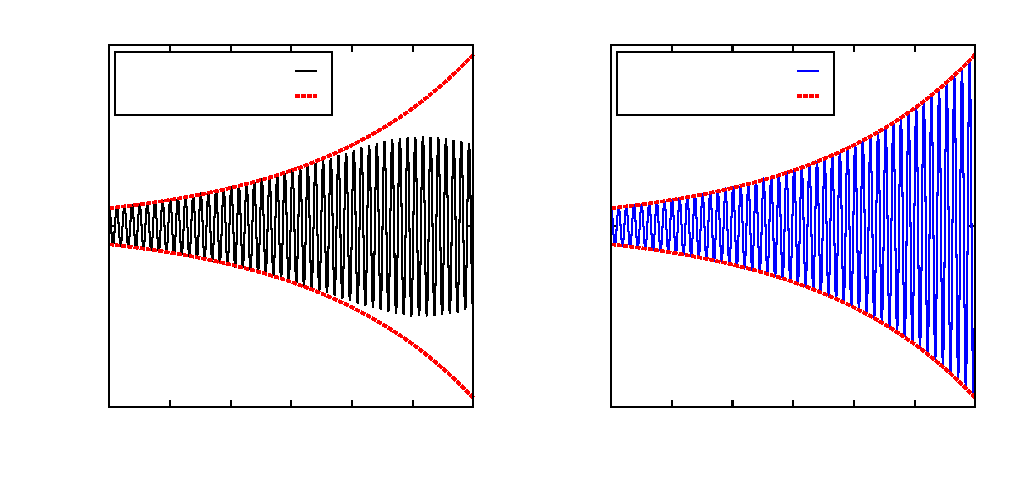
\includegraphics{swing_sim}}%
    \gplfronttext
  \end{picture}%
\endgroup
}
% }

% A note on the applicability of Floquet theory to the swing:\\
% \begin{itemize}
% \item The original EOM is \emph{not} linear.
% \item We can therefore not expect a continued exponential growth.
% \end{itemize}

% \end{frame}


\begin{frame}
\frametitle{}

\end{frame}

\begin{frame}
\frametitle{Bibliography}

\begin{flushleft}
\footnotesize
\begin{itemize}
\item
Burns, J.A. (1970). \textit{More on Pumping a Swing}. Am. J. Phys. \textbf{38}, 920-2

\vspace{-4pt}\item
Ko, C.H., and Takahashi, J.S. (2006). \textit{Molecular components of the
mammalian circadian clock}. Hum. Mol. Genet. R271-7.

\vspace{-4pt}\item
Konopka, R.J., and Benzer, S. (1971). \textit{Clock Mutants of Drosophila
melanogaster}. \textbf{68}, 2112–2116.

\vspace{-4pt}\item
Partch, C.L., Green, C.B., Takahashi (2014).
\textit{Molecular architecture of the mammalian circadian clock}. Trends Cell
Biol. \textbf{24}, 90–99.

\vspace{-4pt}\item
Pfeuty, B., Thommen, Q., and Lefranc, M. (2011). \textit{Robust Entrainment of
Circadian Oscillators Requires Specific Phase Response Curves}.

\vspace{-4pt}\item
Rosato, E., Tauber, E., and Kyriacou, C.P. (2006). \textit{Molecular genetics
of the fruit-fly circadian clock}. Eur. J. Hum. Genet. \textbf{14},
729–738.

\vspace{-4pt}\item
Strub, D.C. (2009). \textit{How do children swing?}  M.Eng. thesis, University
of Bristol, Dept. of Eng. Math.%ematics

\vspace{-4pt}\item
Tea, P.L. Jr. and Falk, H. (1968). \textit{Pumping on a Swing}. Am. J. Phys. 
\textbf{36}, 1165-6

\vspace{-4pt}\item
Ward, M.J. \textit{Basic Floquet Theory}
(http://www.math.ubc.ca/\~{}ward/teaching/m605/every2\_floquet1.pdf).
\end{itemize}
\end{flushleft}
\end{frame}

% \begin{frame}
% \frametitle{Sample frame}
%  \begin{columns}[c]
% \column{.4\textwidth} % Left column and width
% Text here.
% \begin{itemize}
%     \item Individual points.
%     \item Feel free to remove this list.
% \end{itemize}
% \column{.6\textwidth} % Right column and width
% This slide has two columns
% \begin{figure}
% %\includegraphics[width=1\textwidth]{}
% % \caption{}
% \end{figure}
% \end{columns}
% \end{frame}

\end{document}

%  LocalWords:  EOM Floquet
